% ============================================================
% 6. Storyboards
% ============================================================
\chapter{Storyboards}\label{ch:storyboards}

The interface follows an intentionally \emph{aseptic and minimal} style: the
visual appearance is not part of the evaluation, while the interaction logic
must exchange only beans (DTO) with the controllers. Each screen is available
in two themes: \emph{colour} and \emph{black-and-white} (high contrast) for
accessibility.

\begin{figure}[H]
\centering
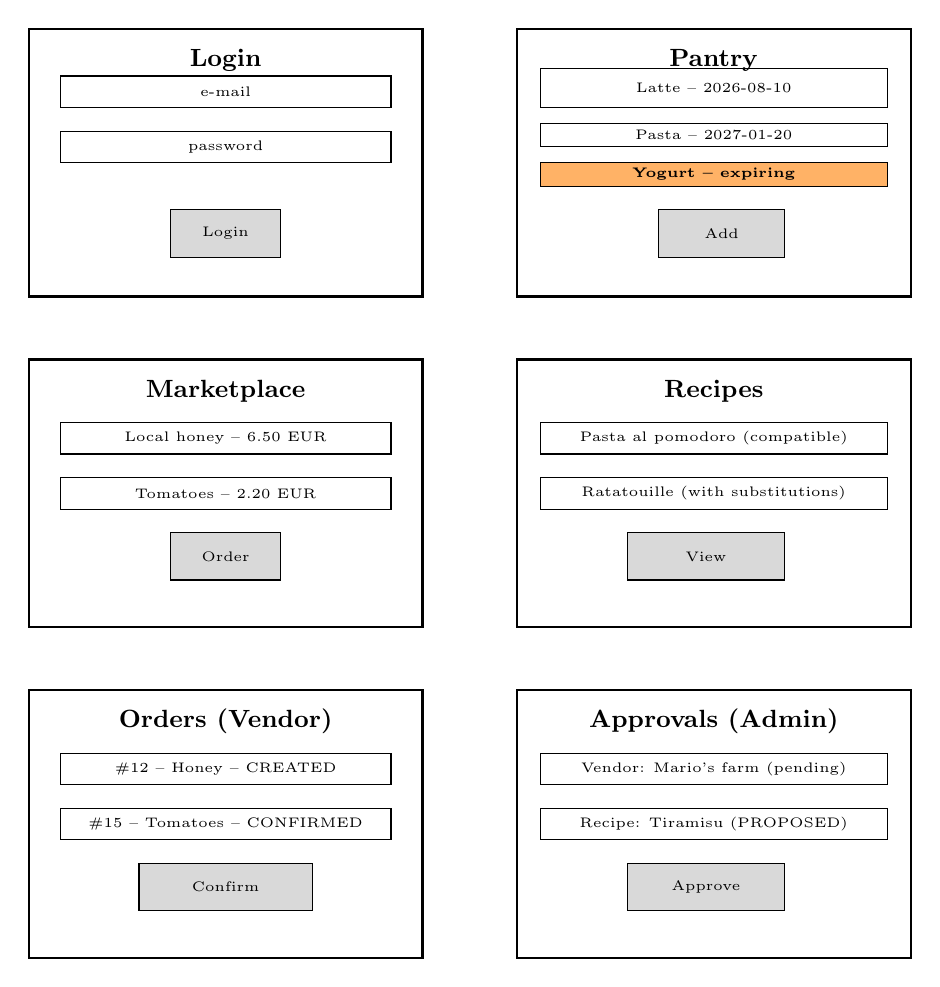
\begin{tikzpicture}[x=1cm,y=1cm]
% Login
\draw[thick] (0,0) rectangle (5,3.4);
\node at (2.5,3.0) {\small\textbf{Login}};
\draw (0.4,2.4) rectangle (4.6,2.8);
\node at (2.5,2.6) {\tiny e-mail};
\draw (0.4,1.7) rectangle (4.6,2.1);
\node at (2.5,1.9) {\tiny password};
\draw[fill=gray!30] (1.8,0.5) rectangle (3.2,1.1);
\node at (2.5,0.8) {\tiny Login};
% Pantry
\draw[thick] (6.2,0) rectangle (11.2,3.4);
\node at (8.7,3.0) {\small\textbf{Pantry}};
\draw (6.5,2.4) rectangle (10.9,2.9);
\node at (8.7,2.65) {\tiny Latte -- 2026-08-10};
\draw (6.5,1.9) rectangle (10.9,2.2);
\node at (8.7,2.05) {\tiny Pasta -- 2027-01-20};
\draw[fill=orange!60] (6.5,1.4) rectangle (10.9,1.7);
\node at (8.7,1.55) {\tiny \textbf{Yogurt -- expiring}};
\draw[fill=gray!30] (8.0,0.5) rectangle (9.6,1.1);
\node at (8.8,0.8) {\tiny Add};
% Marketplace
\draw[thick] (0,-4.2) rectangle (5,-0.8);
\node at (2.5,-1.2) {\small\textbf{Marketplace}};
\draw (0.4,-2.0) rectangle (4.6,-1.6);

\node at (2.5,-1.8) {\tiny Local honey -- 6.50 EUR};
\draw (0.4,-2.7) rectangle (4.6,-2.3);

\node at (2.5,-2.5) {\tiny Tomatoes -- 2.20 EUR};
\draw[fill=gray!30] (1.8,-3.6) rectangle (3.2,-3.0);
\node at (2.5,-3.3) {\tiny Order};
% Recipes
\draw[thick] (6.2,-4.2) rectangle (11.2,-0.8);
\node at (8.7,-1.2) {\small\textbf{Recipes}};
\draw (6.5,-2.0) rectangle (10.9,-1.6);
\node at (8.7,-1.8) {\tiny Pasta al pomodoro (compatible)};
\draw (6.5,-2.7) rectangle (10.9,-2.3);
\node at (8.7,-2.5) {\tiny Ratatouille (with substitutions)};
\draw[fill=gray!30] (7.6,-3.6) rectangle (9.6,-3.0);
\node at (8.6,-3.3) {\tiny View};
% Orders (vendor)
\draw[thick] (0,-8.4) rectangle (5,-5.0);
\node at (2.5,-5.4) {\small\textbf{Orders (Vendor)}};
\draw (0.4,-6.2) rectangle (4.6,-5.8);
\node at (2.5,-6.0) {\tiny \#12 -- Honey -- CREATED};
\draw (0.4,-6.9) rectangle (4.6,-6.5);
\node at (2.5,-6.7) {\tiny \#15 -- Tomatoes -- CONFIRMED};
\draw[fill=gray!30] (1.4,-7.8) rectangle (3.6,-7.2);
\node at (2.5,-7.5) {\tiny Confirm};
% Admin approvals
\draw[thick] (6.2,-8.4) rectangle (11.2,-5.0);
\node at (8.7,-5.4) {\small\textbf{Approvals (Admin)}};
\draw (6.5,-6.2) rectangle (10.9,-5.8);
\node at (8.7,-6.0) {\tiny Vendor: Mario's farm (pending)};
\draw (6.5,-6.9) rectangle (10.9,-6.5);
\node at (8.7,-6.7) {\tiny Recipe: Tiramisu (PROPOSED)};
\draw[fill=gray!30] (7.6,-7.8) rectangle (9.6,-7.2);
\node at (8.6,-7.5) {\tiny Approve};
\end{tikzpicture}
\caption{Minimal storyboards (colour theme): login, pantry with expiry
warning, marketplace, recipes, vendor orders and admin approvals.}
\label{fig:storyboards}
\end{figure}

\section{State of the system}
Every screen makes the system state explicit: the current view, the clickable
actions, and the output area. Buttons are rendered with a grey fill to expose
the affordance of every interaction point. The navigation is linear: \emph{Login}
$\rightarrow$ \emph{Home} $\rightarrow$ \emph{Pantry / Recipes / Marketplace},
with role-based entry points (vendor, nutritionist, administrator).
